%
% Draft  document bundles.tex
% Notes on genetic analysis of ab32 and ab20 skin and wool data
%
 
\documentclass[titlepage]{article}  % Latex2e
\usepackage{graphicx,lscape,subfigure}
\usepackage{bm,longtable}
\usepackage{textcomp}
\usepackage{tikz}
 

\title{ Compound follicles in Merino sheep and fibre diameter}
\author{Neville Jackson , Paul Swan, and Jim Watts}
\date{26 Oct 2018} 

 
\begin{document} 
 
\maketitle      
\tableofcontents


\clearpage
\section{Introduction} 
We are interested in knowing how the various types of follicles found in a trio group vary in fibre diameter. There is ample data in diameter of fibres from primary follicles and secondary follicles, for example Carter(1968)~\cite{cart:68} documents mean Dp and Ds for a wide range of sheep breeds. For the Australian Merino strains in Carter's survey, Dp was larger than Ds by amounts varying from -0.6 to 3 microns for fine-wool strains, 4 to 7 microns for medium wool strains, and 7 to 8 microns for strong wool strains. Another way of expressing this is to say that the ratio Dp/Ds varied from 0.9 up to 1.4. Carter's survey did not include data on modern SRS Merinos. A full comparison, including modern SRS data can be found in Jackson(2017)~\cite{jack:17b}

What is much less avilable is data on the diameters of the various types of secondary follicles and their fibres.  Merino sheep have an S/P ratio greater than 10, and up to 40, the Merino-derived breeds are around 10, and all other breeds have S/P ration of 3 to 7. This very substantial difference has been achieved by forming compound follicles (Hardy and Lyne(1956)~\cite{hard:56} ). The cell biology mechanism behind formation of compound follicles has been explained by Moore et al (1998)~\cite{moor:98}. It involves a population of pre-papilla cells which aggregate at follicle sites in the developing foetal skin. The numbers of papilla cells which aggregate at each site determine the size of the follicle that develops and the diameter of the fibre that it grows. If there are pre-papilla cells left over after all sites have been used, they form extra follicles by branching from existing follicles. Merino sheep have lots of pre-papilla cells and form many branching follicles, mostly secondary follicles, but branching primary follicles have also been observed. There is a small amount of data linking papilla cell number to fibre diameter collected by Dr Philip Moore. These have been re-presented and re-analysed in Jackson and Moore(2018)~\cite{jamo:18} where Figure 4 on page 10 shows quite clearly that fibre diameter is related to number of papilla cells per follicle.

Apart from that, we have just one small study of the number of branches in compound follicles. We are going to attempt here to see if the number of branches in a compound follicle influences fibre diameter.

\section{ Sheep population studied}
Data from CSIRO sheep breeding experiments (AB16a and AB17 in CSIRO jargon) are utilised.  These are all medium and fine wool Merino sheep. These experiments were started by Dr Alex Fraser in 1954. They consisted of 2 lines of medium Merino sheep selected for high and low S/P ratio, and two lines of fine Merino sheep selected for high and low primary follicle density. There is a writeup by Rendel and Nay(1978)~\cite{rend:78}

From the 1971 drop in the above 4 selection lines six male and six female sheep were chosen at random, for detailed study of compound follicles. So 12 sheep from each of 4 selected lines , making a total of 48 sheep.


\section{Traits measured}
Biopsy samples were serial sectioned down to sebaceous gland level. Sections were stained with Haematoxylin, Eosin and picric acid.  A section was chosen, as near to the skin surface as possible, so that fibres could be seen emerging from a common root sheath.  Counts were made of the numbers of fibres emerging from a follicle, for a sample of both primary and secondary follicles. It was not possible to determine which fibre was emerging from the secondary original follicle.

Observations were also available , on the same 48 sheep, of follicle number per unit area (Fn), S/P ratio (Fr), and primary follicle number per unit area (Fp). Average fibre diameter (Diam) by the airflow technique was also available.


\section{Statistical techniques}
Fibre counts were summarized as the relative frequency of follicles with various numbers of emerging fibres, and as the relative frequency of fibres emerging from follicles of various bundle sizes. 

The mean size ( ie number of branches) of secondary follicles was calculated in the usual mannar summing the products of class frequencies and class values.

The regression of average fibre diameter on mean size of secondary follicles was calculated with and without additional predictor variables Fn, Fr, and Fp, using the R function {\em lm()}. The R statistical software~\cite{rprog:13} is free and open source software and is available for Windows, Mac, and Linux systems. Using additional predictor variables enables us to study the effect of bundle size on fibre diameter  as a partial regression holding other variables constant. 

\section{Results}
The difference between the four selected lines in the usual skin measurements ( Fn, Fr, and Fp) are shown in Table~\ref{tab:meanskin}
% latex table generated in R 3.4.2 by xtable 1.8-2 package
% Sun Mar  4 19:57:01 2018
\begin{table}[ht]
\centering
\caption{Means of follicle number per unit area(Fn), S/P ratio (Fr) and primary follicle number per unit area (Fp),for 6 sheep of each sex,  representing the four selection lines Fr+, Fr-, Fp+, Fp-.}
\vspace{0.1in}
\label{tab:meanskin}
\begin{tabular}{rrrrrrrr}
  \hline
  Selection Line & Sex & Mean Fn & Mean Fr & Mean Fp  \\ 
  \hline
   Fr+ & ram &  109.4 & 37.3 & 2.87  \\ 
   Fr+ & ewe & 105.6  & 40.2 & 2.63  \\ \hline
   Fr- & ram &  54.5 &  12.5 & 4.07  \\
   Fr- & ewe &  45.9 &  11.8 & 3.57  \\ \hline
   Fp+ & ram &  69.5 &  14.0 & 4.63  \\
   Fp+ & ewe  & 65.2 &  12.9 & 4.65  \\ \hline
   Fp- & ram  & 58.8 &  28.3 & 2.05  \\
   Fp- & ewe  & 49.8 & 25.1  & 1.9  \\ 
   \hline
\end{tabular}
\end{table}


One can see that there has been a substantial direct response to selection in all four lines, and that there have been correlated changes in the unselected traits.

The counts of fibres emerging from common follicle root sheaths are summarized in Table~\ref{tab:freqfoll}
% latex table generated in R 3.4.2 by xtable 1.8-2 package
% Sun Mar  4 19:57:01 2018
\begin{table}[ht]
\small
\centering
\caption{Frequency of primary and secondary compound follicles of various sizes  for six sheep of each sex representind the four selected lines Fr+, Fr-, Fp+, and Fp-}
\vspace{0.1in}
\label{tab:freqfoll}
\begin{tabular}{rrrrrrrrr}
  \hline
  Follicle & & & & & & & & \\
  size & Fr+ ram & Fr+ ewe & Fr- ram & Fr- ewe & Fp+ ram & Fp+ ewe &  Fp- ram  & Fp- ewe  \\ 
  \hline
 Primary & & & & & & & & \\
 follicles: & & & & & & & & \\
  1 & 93.44 & 95.08 & 97.67 & 98.10 & 99.321 & 98.19 & 97.38 & 99.07 \\
  2 & 4.73  & 2.36  & 0.31  & 0.0   & 0.79   & 0.33  & 1.26  & 0.0   \\
  3 & 1.19  & 0.0   & 0.72  & 1.41  & 0.0    & 0.36  & 0.67  & 0.0  \\
  4 & 0.0   & 1.28  & 1.29  & 0.0   & 0.0    & 0.0   & 0.7   & 0.0  \\
  5 & 0.0   & 0.0   & 0.0   & 0.0   & 0.0    & 0.4   & 0.0   & 0.93  \\
  6 & 0.64  & 0.0   & 0.0   & 0.49  & 0.0    & 0.36  & 0.0   & 0.0  \\
  7 & 0.0   & 1.28  & 0.0   & 0.0   & 0.0    & 0.36  & 0.0   & 0.0  \\
   \hline
  Secondary & & & & & & & & \\
 follicles : & & & & & & & & \\
  1 & 36.1  & 39.95  & 30.21  & 30.97  & 42.67  & 36.68  & 49.00  & 62.63 \\
  2 & 23.81 & 20.15  & 24.34  & 23.52  & 23.55  & 23.80  & 21.43  & 18.49 \\
  3 & 15.28 & 15.00  & 24.16  & 19.42  & 19.65  & 17.90  & 14.04  & 7.85  \\
  4 & 10.84 & 11.03  & 15.51  & 14.41  & 9.09  & 12.38  & 7.91  & 6.59  \\
  5 & 5.34  & 2.94  &  3.24  &  6.92  & 3.62  & 6.13  &  3.29  &  2.14  \\
  6 & 3.66  &  4.31  & 1.41  & 2.09  &  0.87  & 1.93  &  2.11  &  0.82  \\
  7 & 1.83  & 1.93  & 0.83  & 1.25  & 0.31  & 0.53  & 0.81  & 0.68  \\
  8 & 0.92  & 0.88  & 0.25  & 0.45  & 0.082  & 0.37 & 0.64  & 0.37  \\
  9 & 0.70  & 1.14  & 0.00  & 0.58  & 0.08  & 0.15  & 0.55  & 0.23  \\
 10 & 0.41  & 1.16  & 0.06  & 0.14  & 0.00 & 0.15  & 0.19  & 0.21  \\
 11 & 0.58  & 0.50  & 0.00  & 0.00 &  0.00 &  0.00 &  0.057  & 0.00 \\
 12 & 0.24  & 0.42  & 0.00  & 0.32  & 0.082  & 0.00 & 0.00 & 0.00 \\
 13 & 0.043 & 0.41  & 0.0  & 0.0  & 0.0  & 0.0  & 0.0  & 0.0  \\
 14 & 0.14 & 0.0  &  0.0  & 0.0  & 0.0  & 0.0  & 0.0  & 0.0  \\
 15 & 0.0  & 0.0  &  0.0  & 0.0  & 0.0  & 0.0  & 0.0  & 0.0  \\
 16 & 0.0 & 0.12 & 0.0  & 0.0  & 0.0  & 0.0  & 0.0  & 0.0  \\
 17 & 0.087 & 0.11 & 0.0  & 0.0  & 0.0  & 0.0  & 0.0  & 0.0  \\
 25 & 0.043 & 0.0 & 0.0  & 0.0  & 0.0  & 0.0  & 0.0  & 0.0  \\ 
   \hline
\end{tabular}
\end{table}


Differences between the selected lines are not immediately obvious. There is a strain difference, the Fp+ and Fp- sheep are finewool Merinos and they have a higer proportion of single fibre follicles, both primary and secondary. Also the Fr+ selected line tend to have a higer proportion of very highly branched follicles than the Fr- line. 

To see the differences more clearly we compute the mean secondary follicle size for each of the selected line x sex groups. These are given in Table~\ref{tab:meansize}, along with the mean fibre diameter for each group.
% latex table generated in R 3.4.2 by xtable 1.8-2 package
% Sun Mar  4 19:57:01 2018
\begin{table}[ht]
\centering
\caption{Mean size (number of branches) of secondary follicles and mean fibre diameter, for six sheep of each sex representing the four selection lines Fr+, Fr-, Fp+, and Fp-.} 
\vspace{0.1in}
\label{tab:meansize}
\begin{tabular}{rrrr}
  \hline
  Selection Line & Sex & Mean Bundle size & Mean Fibre Diameter  \\ 
  \hline
   Fr+ & ram &  4.30 & 14.63  \\ 
   Fr+ & ewe & 4.67  & 15.60   \\ \hline
   Fr- & ram &  3.19 &  17.65   \\
   Fr- & ewe &  3.71 &  20.15   \\ \hline
   Fp+ & ram &  2.91 &  15.92   \\
   Fp+ & ewe  & 3.30 &  17.32   \\ \hline
   Fp- & ram  & 3.27 &  23.00   \\
   Fp- & ewe  & 2.78 & 19.63   \\ 
   \hline
\end{tabular}
\end{table}


To see the relationship we need to plot the data of Table~\ref{tab:meansize}. We do this in Figure~\ref{fig:1617bundledia}
%\documentclass{article}
%\usepackage{graphicx,subfigure}
%\begin{document}

\begin{figure}[!h]
  \centering
   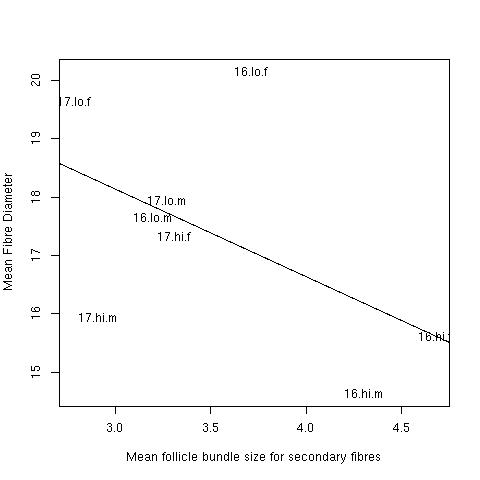
\includegraphics[width=1.0\textwidth]{1617bundledia.png}
  \caption{Plot of mean follicle bundle size for secondary fibres against mean fibre diameter for six sheep of each sex representing the four selection lines Fr+, Fr-, Fp+, Fp-. The solid line is a regression of diameter on bundle size ( Diam = 22.62 - 1.497 * Size). The multiple correlation squared is 0.27. The regression is not significant.}
  \label{fig:1617bundledia}
\end{figure}

%\end{document}


So we have a suggestion of a relationship, but it is not significant. 

It is possible that some other variables are involved in determining diameter. To look into this we will add other variables to the regression. We will look at overall density (Fn), S/P ratio (Fr), and primary density (Fp).

We added, in turn, Fn, Fr, and Fp to the regression fit of diameter on mean secondary follicle bundle size.  The result is shown in Table~\ref{tab:aovreg}
% latex table generated in R 3.4.2 by xtable 1.8-2 package
% Tue Oct 23 20:42:03 2018
\begin{table}[ht]
\caption{Estimates of partial regression coefficients for regression of fibre diameter on mean secondary follicle bundle size and on additional variables Fn, Fr, and Fp}
\label{tab:aovreg}
\centering
\begin{tabular}{rrrrr}
  \hline
 & \multicolumn{4}{l}{Regression of Fibre Diameter  on Secondary bundle size (MeanSc)}  \\
 & Estimate & Std. Error & t value & Pr($>$$|$t$|$) \\ 
(Intercept) & 22.6220 & 3.6060 & 6.27 & 0.0008 \\ 
  MeanSc & -1.4973 & 1.0091 & -1.48 & 0.1884 \\ 
   \hline
 & \multicolumn{4}{l}{Regression of Diameter on MeanSc and MeanFn} \\
 & Estimate & Std. Error & t value & Pr($>$$|$t$|$) \\
(Intercept) & 19.1615 & 1.6553 & 11.58 & 0.0001 \\ 
  MeanSc & 1.5368 & 0.7096 & 2.17 & 0.0826 \\ 
  MeanFn & -0.1033 & 0.0193 & -5.35 & 0.0031 \\ 
   \hline
 & \multicolumn{4}{l}{Regression of Diameter on MeanSc and MeanFr} \\
 & Estimate & Std. Error & t value & Pr($>$$|$t$|$) \\
(Intercept) & 21.6063 & 4.1197 & 5.24 & 0.0033 \\ 
  MeanSc & -0.8661 & 1.4530 & -0.60 & 0.5771 \\ 
  MeanFr & -0.0529 & 0.0831 & -0.64 & 0.5520 \\ 
   \hline
 & \multicolumn{4}{l}{Regression of Diameter on MeanSc and MeanFp} \\
 & Estimate & Std. Error & t value & Pr($>$$|$t$|$) \\
(Intercept) & 24.9256 & 4.7291 & 5.27 & 0.0033 \\ 
  MeanSc & -1.6723 & 1.0655 & -1.57 & 0.1773 \\ 
  MeanFp & -0.5120 & 0.6478 & -0.79 & 0.4651 \\ 
   \hline
 & \multicolumn{4}{l}{Regression of Diameter on MeanFn} \\
 & Estimate & Std. Error & t value & Pr($>$$|$t$|$) \\
(Intercept) & 22.2336 & 1.0840 & 20.51 & 0.0000 \\ 
  MeanFn & -0.0699 & 0.0147 & -4.74 & 0.0032 \\ 
   \hline

\end{tabular}
\end{table}


Table~\ref{tab:aovreg} shows that the regression of diameter on Fn is significant, both on its own ( last section of table) and in the presence of mean secondary bundle size.  It also shows that regression of diameter on mean secondary bundle size is not significant on its own ( first section of table) but is marginally significant ( 8 percent probability) in the presence of Fn. The othe variables had no significant relationship with diameter.

We can illustrate this multiple regression of diameter on secondary bundle size and Fn by plotting the fitted value ( ie the diameter estimated from the multiple regression equation) against the actual diameter, for out eight data points. This is shown in Figure~\ref{fig:multireg}
%\documentclass{article}
%\usepackage{graphicx,subfigure}
%\begin{document}

\begin{figure}[!h]
  \centering
   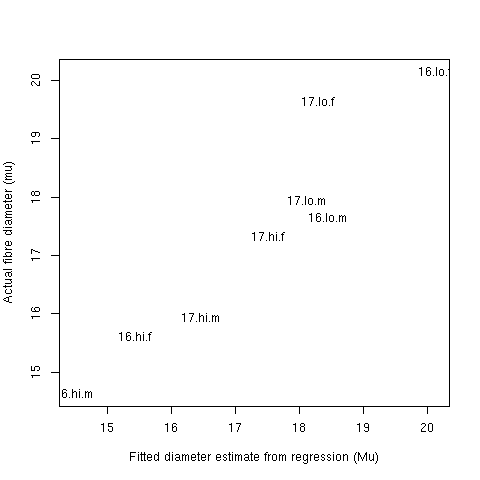
\includegraphics[width=1.0\textwidth]{1617multireg.png}
  \caption{Plot of estimated diameter against actual diameter for the multiple regression of diameter in smean secondary follicle bundle size and Fn.  The points are means of six sheep of each sex representing the four selection lines Fr+, Fr-, Fp+, Fp-. The regression equation is  Diam = 19.16 - 0.103 * Fn + 1.536 * Size. The multiple correlation squared is 0.89. The regression is significant.}
  \label{fig:multireg}
\end{figure}

%\end{document}


That is a much better fit than Figure~\ref{fig:1617bundledia}. The $R^{2}$ value has increased from 0.27 to 0.89.

To prove that the improvement is not all due to adding Fn, we look at the regression of diameter on Fn alone. This is the last section in Table~\ref{tab:aovreg}. The $R^{2}$ value here is 0.79. So it is not quite as good without secondary follicle bundle size. Secondary follicle bundle size contributes something when added on top of Fn, but it is only just significant and it only lifts the $R^{2}$ value from 0.79 to 0.89.

\clearpage
\section{Discussion}
We have shown that mean fibre diameter is affected by follicle number per unit area (Fn) and mean secondary follicle bundle size. What does this mean? If we interpret Fn as an indicator of {\em global follicle density} and secondary follicle bundle size as an indicator of {\em local follicle density}, then we can draw the diagram shown in Figure~\ref{fig:diampath} which is a path diagram suggesting a causal model for fibre diameter.
% Graphic for TeX using PGF
% Title: /home/nevj/common/Fleece-biology/diamlen/compoundfoll/Diagram1.dia
% Creator: Dia v0.97.3
% CreationDate: Wed Oct 24 20:20:57 2018
% For: nevj
% \usepackage{tikz}
% The following commands are not supported in PSTricks at present
% We define them conditionally, so when they are implemented,
% this pgf file will use them.
%\begin{document}
%\begin{landscape}
%\label{fig:diampath}
\begin{figure}[!h]
  \centering

\ifx\du\undefined
  \newlength{\du}
\fi
\setlength{\du}{15\unitlength}
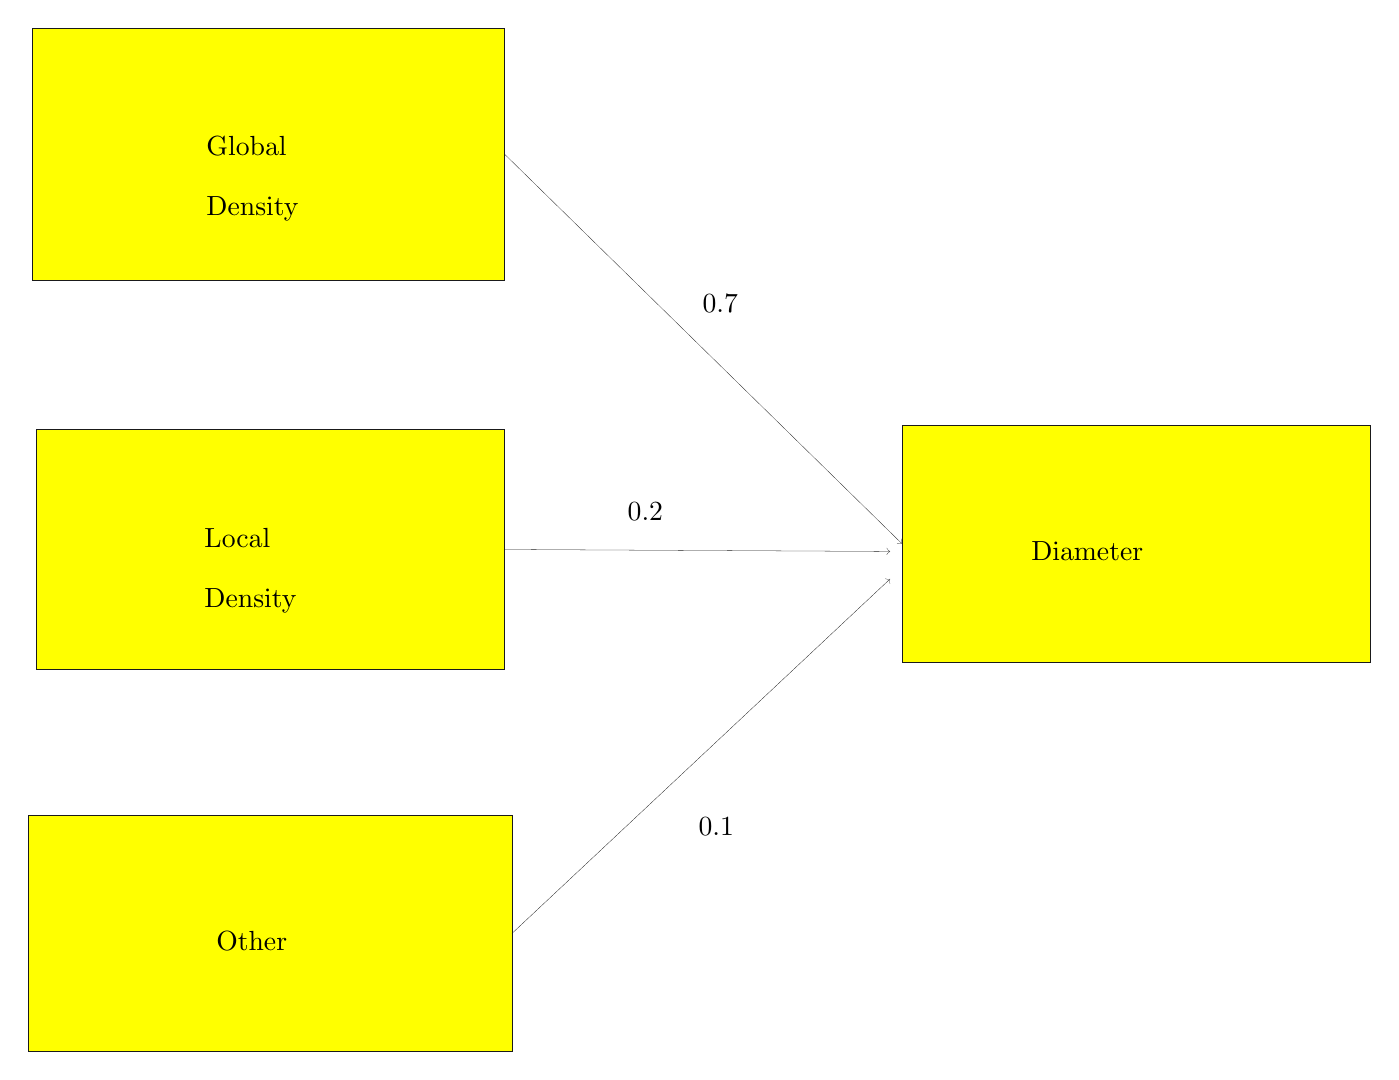
\begin{tikzpicture}
\pgftransformxscale{1.000000}
\pgftransformyscale{-1.000000}
\definecolor{dialinecolor}{rgb}{0.000000, 0.000000, 0.000000}
\pgfsetstrokecolor{dialinecolor}
\definecolor{dialinecolor}{rgb}{1.000000, 1.000000, 1.000000}
\pgfsetfillcolor{dialinecolor}
\pgfsetlinewidth{0.100000\du}
\pgfsetdash{}{0pt}
\pgfsetdash{}{0pt}
\pgfsetmiterjoin
\definecolor{dialinecolor}{rgb}{1.000000, 1.000000, 0.000000}
\pgfsetfillcolor{dialinecolor}
\fill (2.000000\du,1.950000\du)--(2.000000\du,5.150000\du)--(8.000000\du,5.150000\du)--(8.000000\du,1.950000\du)--cycle;
\definecolor{dialinecolor}{rgb}{0.101961, 0.101961, 0.101961}
\pgfsetstrokecolor{dialinecolor}
\draw (2.000000\du,1.950000\du)--(2.000000\du,5.150000\du)--(8.000000\du,5.150000\du)--(8.000000\du,1.950000\du)--cycle;
\pgfsetlinewidth{0.100000\du}
\pgfsetdash{}{0pt}
\pgfsetdash{}{0pt}
\pgfsetmiterjoin
\definecolor{dialinecolor}{rgb}{1.000000, 1.000000, 0.000000}
\pgfsetfillcolor{dialinecolor}
\fill (2.050000\du,7.050000\du)--(2.050000\du,10.100000\du)--(8.000000\du,10.100000\du)--(8.000000\du,7.050000\du)--cycle;
\definecolor{dialinecolor}{rgb}{0.101961, 0.101961, 0.101961}
\pgfsetstrokecolor{dialinecolor}
\draw (2.050000\du,7.050000\du)--(2.050000\du,10.100000\du)--(8.000000\du,10.100000\du)--(8.000000\du,7.050000\du)--cycle;
\pgfsetlinewidth{0.100000\du}
\pgfsetdash{}{0pt}
\pgfsetdash{}{0pt}
\pgfsetmiterjoin
\definecolor{dialinecolor}{rgb}{1.000000, 1.000000, 0.000000}
\pgfsetfillcolor{dialinecolor}
\fill (1.950000\du,11.950000\du)--(1.950000\du,14.950000\du)--(8.100000\du,14.950000\du)--(8.100000\du,11.950000\du)--cycle;
\definecolor{dialinecolor}{rgb}{0.101961, 0.101961, 0.101961}
\pgfsetstrokecolor{dialinecolor}
\draw (1.950000\du,11.950000\du)--(1.950000\du,14.950000\du)--(8.100000\du,14.950000\du)--(8.100000\du,11.950000\du)--cycle;
\pgfsetlinewidth{0.100000\du}
\pgfsetdash{}{0pt}
\pgfsetdash{}{0pt}
\pgfsetmiterjoin
\definecolor{dialinecolor}{rgb}{1.000000, 1.000000, 0.000000}
\pgfsetfillcolor{dialinecolor}
\fill (13.050000\du,7.000000\du)--(13.050000\du,10.000000\du)--(19.000000\du,10.000000\du)--(19.000000\du,7.000000\du)--cycle;
\definecolor{dialinecolor}{rgb}{0.101961, 0.101961, 0.101961}
\pgfsetstrokecolor{dialinecolor}
\draw (13.050000\du,7.000000\du)--(13.050000\du,10.000000\du)--(19.000000\du,10.000000\du)--(19.000000\du,7.000000\du)--cycle;
% setfont left to latex
\definecolor{dialinecolor}{rgb}{0.101961, 0.101961, 0.101961}
\pgfsetstrokecolor{dialinecolor}
\node[anchor=west] at (16.025000\du,8.500000\du){};
% setfont left to latex
\definecolor{dialinecolor}{rgb}{0.101961, 0.101961, 0.101961}
\pgfsetstrokecolor{dialinecolor}
\node[anchor=west] at (16.025000\du,8.500000\du){};
% setfont left to latex
\definecolor{dialinecolor}{rgb}{0.101961, 0.101961, 0.101961}
\pgfsetstrokecolor{dialinecolor}
\node[anchor=west] at (14.575000\du,8.600000\du){Diameter};
% setfont left to latex
\definecolor{dialinecolor}{rgb}{0.101961, 0.101961, 0.101961}
\pgfsetstrokecolor{dialinecolor}
\node[anchor=west] at (4.100000\du,3.450000\du){Global };
% setfont left to latex
\definecolor{dialinecolor}{rgb}{0.101961, 0.101961, 0.101961}
\pgfsetstrokecolor{dialinecolor}
\node[anchor=west] at (4.100000\du,4.250000\du){Density};
% setfont left to latex
\definecolor{dialinecolor}{rgb}{0.101961, 0.101961, 0.101961}
\pgfsetstrokecolor{dialinecolor}
\node[anchor=west] at (4.075000\du,8.425000\du){Local};
% setfont left to latex
\definecolor{dialinecolor}{rgb}{0.101961, 0.101961, 0.101961}
\pgfsetstrokecolor{dialinecolor}
\node[anchor=west] at (4.075000\du,9.225000\du){Density};
% setfont left to latex
\definecolor{dialinecolor}{rgb}{0.101961, 0.101961, 0.101961}
\pgfsetstrokecolor{dialinecolor}
\node[anchor=west] at (4.225000\du,13.550000\du){Other};
\pgfsetlinewidth{0.100000\du}
\pgfsetdash{}{0pt}
\pgfsetdash{}{0pt}
\pgfsetbuttcap
{
\definecolor{dialinecolor}{rgb}{0.101961, 0.101961, 0.101961}
\pgfsetfillcolor{dialinecolor}
% was here!!!
\pgfsetarrowsend{to}
\definecolor{dialinecolor}{rgb}{0.101961, 0.101961, 0.101961}
\pgfsetstrokecolor{dialinecolor}
\draw (8.000000\du,3.550000\du)--(13.050000\du,8.500000\du);
}
\pgfsetlinewidth{0.100000\du}
\pgfsetdash{}{0pt}
\pgfsetdash{}{0pt}
\pgfsetbuttcap
{
\definecolor{dialinecolor}{rgb}{0.101961, 0.101961, 0.101961}
\pgfsetfillcolor{dialinecolor}
% was here!!!
\pgfsetarrowsend{to}
\definecolor{dialinecolor}{rgb}{0.101961, 0.101961, 0.101961}
\pgfsetstrokecolor{dialinecolor}
\draw (8.000000\du,8.575000\du)--(12.900000\du,8.600000\du);
}
\pgfsetlinewidth{0.100000\du}
\pgfsetdash{}{0pt}
\pgfsetdash{}{0pt}
\pgfsetbuttcap
{
\definecolor{dialinecolor}{rgb}{0.101961, 0.101961, 0.101961}
\pgfsetfillcolor{dialinecolor}
% was here!!!
\pgfsetarrowsend{to}
\definecolor{dialinecolor}{rgb}{0.101961, 0.101961, 0.101961}
\pgfsetstrokecolor{dialinecolor}
\draw (8.100000\du,13.450000\du)--(12.900000\du,8.950000\du);
}
% setfont left to latex
\definecolor{dialinecolor}{rgb}{0.101961, 0.101961, 0.101961}
\pgfsetstrokecolor{dialinecolor}
\node[anchor=west] at (10.400000\du,5.450000\du){0.7};
% setfont left to latex
\definecolor{dialinecolor}{rgb}{0.101961, 0.101961, 0.101961}
\pgfsetstrokecolor{dialinecolor}
\node[anchor=west] at (9.450000\du,8.100000\du){0.2};
% setfont left to latex
\definecolor{dialinecolor}{rgb}{0.101961, 0.101961, 0.101961}
\pgfsetstrokecolor{dialinecolor}
\node[anchor=west] at (10.300000\du,12.100000\du){};
% setfont left to latex
\definecolor{dialinecolor}{rgb}{0.101961, 0.101961, 0.101961}
\pgfsetstrokecolor{dialinecolor}
\node[anchor=west] at (10.350000\du,12.100000\du){0.1};
\end{tikzpicture}

\caption{Path diagram showing possible causes of fibre diameter variation. The numbers on each path show the proportion of variance explained} 
\label{fig:diampath}
\end{figure}
%\end{landscape}
%\end{document}



So, if we are willing to assume that density variation causes diameter variation, Figure~\ref{fig:diampath} says that 70 percent of diameter variation is globally determined, and anothe 20 percent is locally determined, and the final 10 percent is unexplained. 

Given what we know about the role of  papilla cell numbers in determining fibre diameter (Moore etal (1998)~\cite{moor:98}), the above interpretation is probably incorrect. What it means is that if the papilla cells are shared around over more follicles, then there tend to be less papilla cells per follicle, and therefore finer fibres. The sharing is during follicle development, not while the fibre is growing in an adult functioning follicle. What is being shared is the papilla cells, and there is a global and a local component to that.  We can be quite sure that this is not evidence of competition between follicles for nutrients during fibre growth. 

A few words of caution. Is secondary follicle bundle size really an indicator of local density? Well it is a rough one, when compound follicles have lots of branches the follicles tend to be locally dense. It would be preferable to have some actual counts of local density. 

One might wonder why Fn had a significant diameter effect, but Fr ( S/P ratio) did not. Normally Fn and Fr are highly correlated. In the present dataset the correlation is 0.78. Yet the $R^{2}$ for regression of diameter on secondary follicle bundle size and Fr was only 0.32. We have to  remember that Fr is a measure, not of density, but of the number of follicles in a trio group. The formula for number of follicles in a trio group is $3 + 3Fr$, which , of course, is linearly related to Fr.  The number of follicles in a group is not follicle density, because the area of a trio group can vary. We have no measure of intra-group density in the present dataset, because group area was not measured. Fn will not be the same as intra-group density, because there is connective tissue between the trio groups which is counted in calculating Fn, but would not be counted if intra-group density were measured. In the present data we are approximating intra-group density with secondary follicle bundle size. It is a very rough approximation. 

So the traditional interpretation of Fr, as Fn corrected to an equal Fp and hence to equal body size, might be used with some caution.  It works if Fp ( primary follicle density) is just a measure of growth. There is however a much better interpretation as indicated above. 

We need to be aware too, that this study is a very small amount of data, and that the counts of secondary follicle bundle size were subject to a large sampling error. We were only able to analyse means for the line x sex groups, not individual sheep, because we needed to attenuate some of the errors by averaging.


\clearpage

\begin{thebibliography}{99}

\bibitem{cart:43}
Carter, H.B. (1943) Studies in the biology of the skin and fleece of sheep. CSIRO (Aust) Bull. No. 164

\bibitem{cart:68}
Carter,H.B. (1968) Comparative Fleece Analysis Data for Domestic Sheep. The Principal Fleece Staple Values of Some Recognised Breeds. Agricultural Research Council, 1968


\bibitem{chap:65}
Chapman, R.E. (1965) The ovine arrector pili musculature and crimp formation 
    in wool. In "Biology of the Skin and Hair Growth" Angus and Robertson,
    Sydney, Ed. A.G. Lyne and B.F. Short. pp 201-232

\bibitem{hard:56}
Hardy, M.H. and Lyne, A.G. (1956) The prenatal development of wool follicles in Merino sheep. Aust. J. biol. Sci. 9:423-441

\bibitem{hori:53}
Horio, M. and Kondo, T. (1953) Text. Res. J. 23:373

\bibitem{jack:17}
Jackson, N.(2017) Genetic relationship between skin and wool traits in Merino sheep. Part I Responses to selection and estimates of additive genetic parameters. URL https://github.com/nevillejackson/Fleece-genetics/tree/master/skinandfleeceparameters/ab3220/skinwool1.pdf

\bibitem{jack:17a}
Jackson, N. and Watts, J.E. (2017) What is known about the genetics of wrinkle score in Merino sheep? URL https://github.com/nevillejackson/Fleece-genetics/tree/master/wrinkle/wrinkle.pdf

\bibitem{jack:75}
Jackson, N., Nay T. and Turner, Helen Newton (1975) Response to selection
    in Australian Merino sheep. VII Phenotypic and genetic parameters for
    some wool follicle characteristics and their correlation with wool and
    body traits. Aust. J. Agric. Res. 26:937-57

\bibitem{jack:15}
Jackson, N. and Watts, J.E. (2016) Staple crimp formation in the fleece of Merino sheep. 
Report available from the authors as a pdf document.

\bibitem{jack:16a}
Jackson, N.  and Watts J.E. (2016) Can we predict intrinsic fibre curvature from follicle curvature score? Report available from the author as a pdf document.

\bibitem{jack:15b}
Jackson, N. (2015) An Overview of the R package dmm.
    From http://cran.r-project.org/package=dmm
    Or https://github.com/cran/dmm

\bibitem{jack:86}
Jackson, N. Lax, J. and Wilson, R.L.(1986) Sex and selection for fleece weight in Merino sheep. Zeitschrift fur Tierzuchtung und Zuchtungsbiologie. Bd. 103:97-115

\bibitem{jack:17b}
Jackson, N. (2017) What are the defining characteristics of a primitive sheep relative to a modern Merino sheep? https://github.com/nevillejackson/atavistic-sheep/tree/master/mev-rewrite/supplementary/primitive/primitive.pdf

\bibitem{jack:18}
Jackson, N. and Watts, J. E. (2018) Does follicle development affect the spatial layout of sheep skin? URL https://github.com/nevillejackson/Fleece-biology/tree/master/skinspace/skinspace.pdf

\bibitem{jamo:18}
Jackson, N. and Moore, G.P.M (2018) Dynamics of pre-papilla cell numbers in sheep foetus and effect on follicle development. URL https://github.com/nevillejackson/Fleece-biology/tree/master/pre-papilla-cells/ppcell.pdf

\bibitem{lync:97}
Lynch, M. and Walsh, B. (1997) Genetics and Analysis of Quantitative Traits. Sinauer, Massachusetts, USA, 1997

\bibitem{moor:89}
Moore, G.P.M, Jackson, N. and Lax, J. (1989) Evidence of a unique developmental mechanism specifying both wool follicle density and fibre size in sheep selected for single skin and fleece characters. Genet. Res. Camb.  53:57-62

\bibitem{moor:98}
Moore, G.P.M., Jackson, N., Isaacs, K., and Brown, G (1998) J. Theoretical Biology 191:87-94

\bibitem{nago:81}
Nagorcka, B.N. (1981) Theoretical mechanism for crimp.
     Aust J. Biol. Sci. 34: 189-209

\bibitem{onio:62}
Onions, W.J. (1962) Wool: an introduction to its properties, varieties, uses
     and production. Ernest Benn limited, London, 1962

\bibitem{rend:78}
Rendel, J.M. and Nay, T. (1978) Selection for high and low ratio and high 
    and low primary density in Merino sheep. 
    Aust. J. Agric. Res. 29:1077-86

\bibitem{rprog:13}
R Core Team (2013). R: A language and environment for statistical
  computing. R Foundation for Statistical Computing, Vienna, Austria.
  ISBN 3-900051-07-0, URL http://www.R-project.org/.

\bibitem{sear:92}
Searle, S.R., Casella, G., and McCullock, C.E. (1992) Variance Components.
    John Wiley and Sons, New York.


\bibitem{swan:93}
Swan, P.G. (1993) Objective measurement of fibre crimp curvature and the bulk compressional properties of Australian wools. PhD Thesis, University of NSW, March 1993 

\bibitem{wats:77}
Watson, N., Jackson, N. and Whiteley, K.J. (1977) Inheritance of the resistance
    to compression property of Austrailian Merino wool and its genetic 
    correlation with follicle curvature and various wool and body 
    characters. Aust. J. Agric. Res. 28:1083-94

\bibitem{wola:14}
Wolak, M.E. (2014) nadiv: an R package to create relatedness matrices for
    estimating non-additive genetic variances in animal models.
    Methods in Ecology and Evolution 3:792-796.

\bibitem{turn:68}
Turner, H.N., Dolling, C.H.S, and Kennedy, J.F. (1968) Response to selection in Australian Merino sheep. I Selection for high clean wool weight with aceiling on fibre diameter and degree of skin wrinkle. Aust.J.agric.Res. 19:79-112

\bibitem{turn:53}
Turner, H.N., Hayman, R.H., Riches, J.H., Roberts, N.F., and Wilson, L.T. (1953) Physical definition of sheep and their fleece for breeding and husbandry studies, with particular reference to Merino sheep. CSIRO Aust. Div. Anim. Hlth. Prod. Divl. Rep. No 4 (Series S.W. -2)

\end{thebibliography}


\end{document}

